\subsection{Instance Representation}
\label{sect:instance}
As discussed in the previous section, all of the PDDL predicates and actions may be
decomposed into a small set of primitives that includes
Robot Actions, Vision Actions, RCC-8 relations, and Observables. 
If this set of primitives is
programmed into the robot cell, then the set of behaviors that the cell is capable of
may be altered through the creation of new PDDL actions and predicates rather than
reprogramming the cell. In addition, these PDDL actions and predicates are independent
of the actual cell's implementation and product vendors. As long as the cell supports the
full set of primitives, it is capable of carrying out the operations without programming.

In order to translate PDDL predicates and actions into robot cell commands, 
the executor needs to have an
understanding of how the predicates and actions are composed. Since this information is
designed to not be hard-coded on the robot, it must be accessible to the running system.
In addition, since the actions and predicates are designed to be expanded upon as
new activities are added to the robot's vocabulary, the information needs to be
accessible in a human friendly form.
%
\begin{figure}[htb!]
\begin{center}
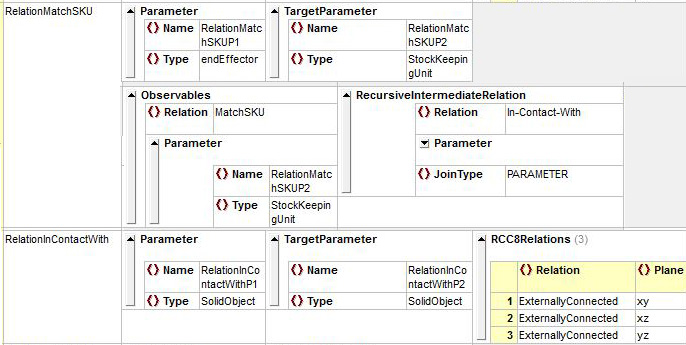
\includegraphics[width=12cm]{images/MatchSKU_ISR.jpg}
\caption{Intermediate State Relation RelationMatchSKU. This is the
implementation of Equation \ref{equation:matchSKU}.}
\label{fig:ISR}
\end{center}
\end{figure}
%
To meet all of these demands, this information is encoded in the Instance Ontology and is automatically entered into the Execution Model's MySQL database. 

The primitives themselves are implemented as simpleTypes in the schema.
In this case, the XML simpleType specifies an enumerated list of terms
that are within the robot and vision system's vocabulary. All of the
ISRs, predicates, and actions are composed of these elements, and these
elements are the only part of the system that is hard-coded onto the
robot.
\subsubsection{Intermediate State Relation}
The structure of the RelationMatchSKU ISR required by Equation \ref{equation:matchSKU} is shown in the XML
representation
depicted in Figure \ref{fig:ISR}. 
Recall from Equation \ref{equation:matchSKU} that this ISR is 
a recursive combination of the Robot ISR \textbf{In-Contact-With} and
the Vision ISR \textbf{MatchSKU}. This is shown in the XML in that
the \textit{RecursiveIntermediateRelation} is instantiated as
\textbf{In-Contact-With} with a single parameter of the end effector
and the \textit{JoinType} of \textit{PARAMETER}. This will cause a determination
of every object that is in contact with the effector. The 
determination of which objects are in contact with the effector
is made through the application of RCC-8 relations as shown in
the bottom part of Figure \ref{fig:ISR}. In this case, three
externally connected relations must be evaluated for each
object.The list of objects in contact
will get passed back as parameters to the \textit{MatchSKU} Vision ISR.
If zero or greater than one objects are passed to \textit{MatchSKU},
an error will be generated. If and only if one object is passed as
a parameter, that object's SKU will be compared against the target
SKU. Thus, from a combination of primitives we are able to determine
if the object being held by the end effector matches the SKU of the
expected object class. This in turn will deliver the truth value
of the predicate \textit{endEffector-has-heldObject()} depicted
in Equation \ref{equation:endEffector-has-heldObject}.  
\subsubsection{Actions}
\textit{CRCLActionTypes} and \textit{VisionActionTypes} are included
in the xml schema and are extensions of the \textit{ActionType} depicted
in Figure \ref{fig:ActionType}. These actions add the list of CRCL commands or observations that are required for the execution of the action. A sample of the CRCL commands for the \textit{place-part} action
are shown in Figure \ref{fig:PlacePartCRCL}. The encoding of all of the
actions is performed in the instance ontology.
